\RequirePackage{fix-cm}
\documentclass[twocolumn]{svjour3}
% DRAFT 1 -- for the first draft discussion (stage after the F3 pilot, 50 validation dishes).
% Full prose: Introduction, Related work, Methods, pilot Results. Discussion as bullet points.
% Blue = planned content (bullets). Red in brackets = open decision for the discussion.

\usepackage{cite}
\usepackage{graphicx}
\usepackage{amsmath}
\usepackage{amssymb}
\usepackage{xcolor}
\usepackage{booktabs}
\usepackage{multirow}
\usepackage{url}
\usepackage{balance}

\newcommand{\plan}[1]{{\color{blue!70!black}#1}}
\newcommand{\open}[1]{\textcolor{red!70!black}{[#1]}}
\graphicspath{{figs/}}

\journalname{Draft 1 -- for discussion}

\begin{document}

\title{How Many Questions Are Enough? Budgeted Questions with Noisy Answers for Calorie Estimation from Meal Photos}
\titlerunning{Budgeted questions for photo-based calorie estimation}

\author{Adam~Soko{\l}owski \and Antoni~Grajek}
\authorrunning{A.~Soko{\l}owski, A.~Grajek}

\institute{A.~Soko{\l}owski, A.~Grajek \at
  Warsaw University of Technology, \open{faculty / institute to confirm}
}

\date{Draft 1 (after the pilot study)}

\maketitle

\begin{abstract}
Vision-language models can estimate the energy content of a meal from a single photograph, but they
cannot see portion size or hidden fat and remain far less accurate than dedicated models. Interactive
systems reduce this error by asking the user for extra information, yet existing work asks many questions
and assumes that the user knows the exact answer. We study a realistic setting in which an application may
ask at most three questions and people answer with error. We define a pool of seven questions answerable
from the Nutrition5k dataset, four simulated users calibrated on studies of human portion estimation, and
five question-selection strategies, including a learned selector driven by the model's uncertainty. A pilot
on 50 validation dishes with Qwen2.5-VL-7B showed reliable structured output (0\% parsing failures), a
photo-only error of 39\% after removing near-empty plates, and an unexpected result: all seven answers
together did not lower the error (43\%). The pilot fixed the protocol for the main experiment, which
evaluates every question subset of size up to three offline. \plan{Main results: to be added after the
full experiment.}
\keywords{calorie estimation \and vision-language models \and clarifying questions \and active feature acquisition \and Nutrition5k}
\end{abstract}

% =====================================================================
\section*{Questions for the first discussion}
\label{sec:questions}
\begin{enumerate}
  \item \textbf{All answers did not help in the pilot} (38.9\% $\rightarrow$ 42.7\% MAPE on 43 dishes).
        Do we treat this as a finding and keep the prompt, or tune the prompt until full information helps?
  \item \textbf{Reference for H1.} If ``all questions'' is not an upper bound, should the share of the
        gain be measured against the per-dish oracle instead?
  \item \textbf{Near-empty plates.} Seven of 50 pilot dishes have under 50\,kcal and raise MAPE from 39\%
        to 85\%. Is excluding them acceptable, or should MAE be the main metric?
  \item \textbf{H4 threshold.} 82\% of dishes get more than 10\% of energy from fat, so the 10\% split is
        not informative. Is a 30\% threshold acceptable?
  \item \textbf{Noise calibration.} $\sigma=0.33$ gives 56\% of answers within $\pm$25\% (the source reports
        about 50\%); keep it, given the grid $\sigma\in\{0.1, 0.33, 0.5\}$?
  \item \textbf{Compute.} The full protocol needs about 116 thousand calls (about 39\,h on our laptop GPU).
        A second model (E5) would double it. Can it move to future work?
\end{enumerate}

% =====================================================================
\section{Introduction}
\label{sec:intro}

Photo-based food logging is one of the most convenient ways to track energy intake, and general-purpose
vision-language models (VLMs) now make it possible without any task-specific training. Their estimates,
however, remain imprecise. On Nutrition5k~\cite{thames2021nutrition5k}, dedicated models reach a calorie
error of 26\% from a single RGB image and 15--19\% with real or predicted
depth~\cite{thames2021nutrition5k,han2023dpf}, whereas zero-shot GPT-4V has a mean absolute percentage
error (MAPE) of 55\%~\cite{tanabe2024calorielava}, and recent commercial models still miss by about 36\%
on standardised photographs~\cite{fridolfsson2025llm}. The gap is not only a matter of model size: the
image itself lacks the information that matters most.

Two sources of error dominate. The first is portion size, because a single overhead photo does not show
the third dimension; volume estimation has long been the weakest stage of image-based dietary
assessment~\cite{lo2020review,vinod2026portion}, and VLMs in particular recognise food volume
poorly~\cite{tanabe2025calorievol}. The second is hidden energy, such as cooking oil, butter and dressings,
which adds many calories while being barely visible~\cite{bhatambarekar2025thesis}. Neither can be fully
recovered from pixels, but both are known to the person who ate the meal.

Asking the user is therefore a natural remedy, and it works. Giving GPT-4o the ingredient masses lowers
its MAPE from about 51\% to 29\%~\cite{bhatambarekar2025thesis}, contextual metadata improves large
multimodal models~\cite{coburn2025lmm}, and an agent that asks its own clarifying questions beats a fixed
question sequence~\cite{bhatambarekar2026agentic}. Not every piece of information is worth asking for,
though: the dish name alone barely changes the error of an image model~\cite{narang2025multimodal}.

Existing interactive work leaves two practical questions open. First, it either asks every question in
a fixed ladder or lets an agent ask without limit, while each extra question adds user burden, and in
dietary assessment lower burden usually comes at the cost of lower accuracy~\cite{hochsmann2020review}. How much accuracy one, two or three questions can buy, and which
questions they should be, has not been measured. Second, answers are taken from the dataset's ground
truth, although people estimate portions poorly: only 35--50\% of their estimates fall within $\pm$25\% of
the true mass~\cite{lucassen2021portion}. It is unknown how much of the reported gain survives realistic
answers, and whether the ranking of useful questions changes. Methods for selecting what to ask under a
cost, studied as active feature acquisition~\cite{aronsson2025afa} and as information-gain-driven
clarification for language models~\cite{kobalczyk2025active,infogain2026clarification}, have not been
applied to this problem.

We address these gaps with three research questions. \textbf{RQ1:} how does the calorie error depend on a
question budget of 0--3? \textbf{RQ2:} does an uncertainty-driven, image-dependent question selector
outperform a fixed order, random choice and a VLM choosing its own questions at the same budget?
\textbf{RQ3:} how do noisy and coarse answers change the value of interaction and the ranking of
questions? We test four hypotheses: two well-chosen questions give at least 70\% of the error reduction of
full information (H1); the learned selector is significantly better than random and fixed-order selection
and not worse than the agent (H2); realistic noise reduces the gain of the grams question by at least 30\%
and makes categorical questions competitive (H3); and the fat question helps most for fat-rich dishes (H4).

Our contributions are an evaluation protocol for budgeted interactive calorie estimation with simulated
users calibrated on human data, error-versus-budget curves and a strategy comparison for an open VLM on
Nutrition5k, and recommendations on which questions are worth asking real users. This draft reports the
protocol and the pilot study that fixed it; the main experiment follows the same protocol.

% =====================================================================
\section{Related work}
\label{sec:related}

\paragraph{Image-based calorie estimation.}
Im2Calories~\cite{meyers2015im2calories} established the recognition--segmentation--volume pipeline and
showed that portion is its hardest stage, a conclusion repeated by later reviews~\cite{lo2020review,vinod2026portion}.
Nutrition5k~\cite{thames2021nutrition5k} provided cafeteria dishes with weighed ingredients and overhead
RGB-D images, and models with predicted depth~\cite{han2023dpf} or richer datasets~\cite{yu2026omnifood8k}
now lead single-image benchmarks. Such models rely on large-scale pre-training that public alternatives do
not match~\cite{andrade2025pretraining}, which makes general-purpose VLMs an attractive alternative.

\paragraph{Multimodal language models for nutrition.}
Fine-tuning LLaVA on Nutrition5k lowers its error below that of GPT-4V~\cite{tanabe2024calorielava}, and
adding an estimated volume to the prompt helps further~\cite{tanabe2025calorievol}. Other systems combine
VLMs with retrieval and conversation~\cite{yao2024caloraify} or with reinforcement-learned
reasoning~\cite{zhu2026foodr1}. Benchmarks of zero-shot models show large errors and a strong dependence on
the model and the prompt~\cite{fridolfsson2025llm,coburn2025lmm,nutrients2026prompt}.

\paragraph{Interaction with the user.}
The closest work evaluates eight multimodal models with a ladder of cues (ingredients, total mass,
ingredient masses) and with an agent that asks its own questions~\cite{bhatambarekar2025thesis,bhatambarekar2026agentic}.
Total mass is the strongest single cue, and agentic questioning beats a fixed sequence. Both studies use
exact answers from the dataset and no question budget; we add both constraints.

\paragraph{Choosing what to ask.}
Active feature acquisition selects, per instance, which features to acquire under a cost; strategies range
from static orders to greedy and reinforcement-learned policies~\cite{aronsson2025afa,schutz2025afabench}.
Language models can supply prior knowledge for this choice, but they plan acquisition sequences
poorly~\cite{perets2026zeroshot}. For clarifying questions, maximising expected information gain improves
task disambiguation~\cite{kobalczyk2025active,infogain2026clarification}, and models rarely ask useful
questions unless trained to do so~\cite{zhang2024clarifying}. We follow the acquisition view and keep the
selector separate from the estimating VLM.

% =====================================================================
\section{Methods}
\label{sec:methods}

Figure~\ref{fig:pipeline} shows the pipeline. For each dish, a strategy chooses up to $B$ questions, a
simulated user answers them, and the VLM estimates the energy from the photo and the answers.

\begin{figure*}[t]
  \centering
  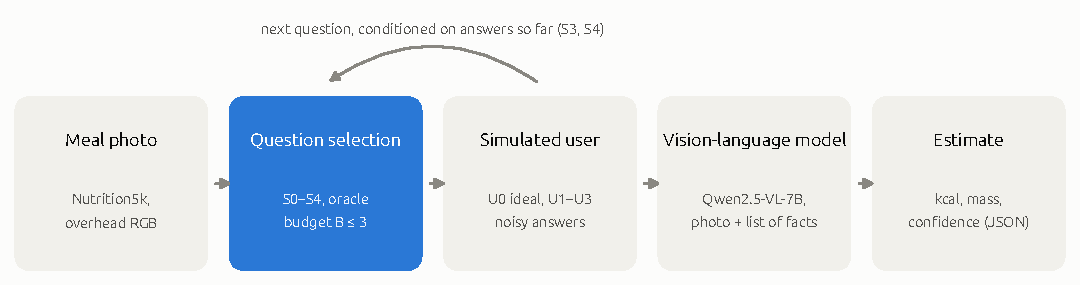
\includegraphics[width=0.9\textwidth]{fig_pipeline}
  \caption{Evaluation pipeline. A strategy selects up to $B\le 3$ questions, a simulated user answers them
  (possibly with error), and the vision-language model estimates energy from the photo and the answers.}
  \label{fig:pipeline}
\end{figure*}

\subsection{Data}
We used Nutrition5k~\cite{thames2021nutrition5k}, which contains real cafeteria dishes with weighed
ingredients and overhead RGB photographs. We downloaded only the overhead images and the metadata (1.46\,GB
instead of about 180\,GB). A validation set of 300 dishes was sampled with a fixed seed from the official
training split and used to fit strategies; the official test split was used for evaluation. After the pilot
(Section~\ref{sec:pilot}) we excluded dishes under 50\,kcal, which left 300 validation and 424 test dishes.

\subsection{Question pool}
Table~\ref{tab:questions} lists the seven questions. Each true answer was derived from the metadata: the
fat and sauce questions use hand-made ingredient lists, and the size categories use the terciles of dish
mass on the validation set ($<$153\,g, 153--288\,g, $>$288\,g), which were shown to the model with the
answer. Answers enter the prompt as an unordered list of facts, so a set of questions defines the prompt
independently of the order in which they were asked.

\begin{table}[t]
  \centering
  \caption{Question pool and the source of the true answer in Nutrition5k.}
  \label{tab:questions}
  \setlength{\tabcolsep}{3pt}
  \begin{tabular}{@{}lp{3.2cm}p{3.1cm}@{}}
    \toprule
    ID & Question & True answer \\
    \midrule
    Q1 & How much did the meal weigh (g)? & total mass \\
    Q2 & Was the portion small, medium or large? & mass tercile \\
    Q3 & Was it fried, or was oil/butter added? & fat ingredient present \\
    Q4 & Was there a sauce or dressing? & sauce ingredient present \\
    Q5 & What is the main ingredient? & heaviest ingredient \\
    Q6 & Please list the ingredients. & ingredient list \\
    Q7 & How many separate items are on the plate? & ingredients $\ge$10\,g \\
    \bottomrule
  \end{tabular}
\end{table}

\subsection{Simulated users}
The ideal user U0 returns the true answers, as in prior work. User U1 perceives mass with a log-normal
error, $m' = m\,e^{\varepsilon}$ with $\varepsilon\sim\mathcal{N}(\mu,\sigma)$; we used $\sigma\in\{0.1, 0.33,
0.5\}$ and a variant with $\mu=0.2$ (over-estimation). The value $\sigma=0.33$ puts 56\% of answers within
$\pm$25\% of the truth, close to the 50\% reported for textual portion descriptions~\cite{lucassen2021portion}.
The size category (Q2) uses the same perceived mass, so the user is consistent. User U2 makes categorical
mistakes with probability $p\in\{0.1, 0.2\}$: an adjacent size category, a flipped yes/no answer, the second
heaviest ingredient, a forgotten ingredient or a count off by one. User U3 answers ``I don't know'' with
probability $q=0.2$, and the question still uses up the budget. Answers were drawn once per dish and user,
so the same user gives the same answer whatever else is asked.

\subsection{Model and prompt}
We used Qwen2.5-VL-7B-Instruct in 4-bit AWQ quantisation, served with vLLM on a single 8\,GB laptop GPU.
The prompt contained the photo, the list of facts and a request for a JSON object with energy (kcal), mass
(g) and a confidence between 0 and 1, decoded at temperature 0. Because the prompt depends only on the set
of questions, we computed predictions for every subset of size at most three ($1+7+21+35=64$ subsets) and
every user variant, and evaluated all offline strategies by lookup. Identical prompts were computed once.

\subsection{Question-selection strategies}
\textbf{S0} uses the photo only. \textbf{S1} chooses questions at random; we report its exact expectation
over all subsets of size $B$. \textbf{S2} asks questions in a fixed order, built greedily on the validation
set to minimise mean error. \textbf{S3} lets the VLM choose the next question itself from the remaining
pool, step by step, given the answers so far. \textbf{S4}, our selector, is a gradient-boosted regressor
(LightGBM) that predicts, for each candidate question, the reduction in the dish's absolute percentage error
when that question is added. Its features describe the model's uncertainty (spread of $K=5$ photo-only
samples at temperature 0.7, stated confidence), the current and photo-only estimates, the answers obtained
so far and the user's noise parameters. S4 picks the question with the largest predicted gain, greedily,
until the budget is used. The \textbf{oracle} chooses, with knowledge of the true energy, the best subset of
size at most $B$ for each dish and is an upper bound.

\subsection{Metrics and statistics}
The main metric is MAPE; we also report MAE (kcal) and the share of estimates within $\pm$20\% of the
truth (acc@20\%). We summarise each strategy by its share of the oracle's gain at the same budget,
$(\mathrm{MAPE}_{S0}-\mathrm{MAPE}_{s})/(\mathrm{MAPE}_{S0}-\mathrm{MAPE}_{\mathrm{oracle}})$, and by the gain
it recovers relative to asking all seven questions. Strategies are compared with the paired Wilcoxon
signed-rank test on per-dish errors, with bootstrap 95\% confidence intervals of the mean difference and
Holm correction within each user variant.

% =====================================================================
\section{Pilot study}
\label{sec:pilot}

Before the main experiment we ran a pilot on 50 validation dishes to check output reliability, the size of
the effect and the computational cost (Table~\ref{tab:pilot}). In an earlier ten-dish demonstration the
3B model anchored on fixed values and became much worse with full information (MAPE 60\% $\rightarrow$ 82\%),
so we continued with the 7B model.

\begin{table}[t]
  \centering
  \caption{Pilot on 50 validation dishes (Qwen2.5-VL-7B-AWQ): MAPE [\%] with the photo only (S0) and with
  all seven answers (U0), and throughput. ``$\ge$50'' excludes the 7 dishes under 50\,kcal.}
  \label{tab:pilot}
  \setlength{\tabcolsep}{3.5pt}
  \begin{tabular}{@{}llrrr@{}}
    \toprule
    Prompt & Dishes & S0 & All 7 & s/call \\
    \midrule
    \multirow{2}{*}{Direct JSON}      & all 50     & 85.1 & 50.8 & \multirow{2}{*}{1.2} \\
                                      & $\ge$50 (43) & 38.9 & 42.7 & \\
    \midrule
    \multirow{2}{*}{Short reasoning}  & all 50     & 88.5 & 67.5 & \multirow{2}{*}{2.8} \\
                                      & $\ge$50 (43) & 46.4 & 53.6 & \\
    \bottomrule
  \end{tabular}
\end{table}

The model returned valid JSON for every call, and no value had to be clamped. A short reasoning field
before the numbers made the estimates worse and more than doubled the time per call, so we used direct
JSON output. Near-empty plates dominated the percentage error (Fig.~\ref{fig:pilot}): an estimate of 150\,kcal for
a dish of about 12\,kcal is an error of over 1000\%, and the seven dishes under
50\,kcal raised the photo-only MAPE from 39\% to 85\%. With these dishes removed, the photo-only error
(39\%) was within the range reported for zero-shot models, but all seven answers together increased it to
43\%, while the median error stayed the same (33\%). The full protocol required about 116 thousand
unique calls, about 39 hours at the measured throughput.

\begin{figure}[t]
  \centering
  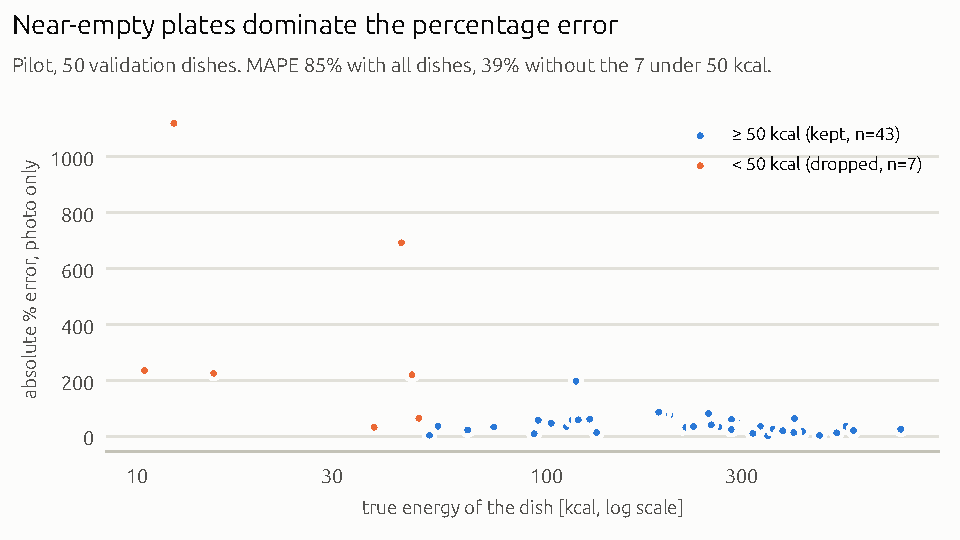
\includegraphics[width=\columnwidth]{fig_pilot_small_plates}
  \caption{Pilot, photo only: absolute percentage error against the true energy of the dish. Dishes under
  50\,kcal (orange) dominate the mean error.}
  \label{fig:pilot}
\end{figure}

% =====================================================================
\section{Planned analyses and expected results}
\label{sec:plan}
\plan{
\begin{itemize}
  \item E1: error versus budget $B=0..3$ for S0--S4 and the oracle, ideal user (RQ1, H1, H2).
  \item E2: the same for U1 (three $\sigma$ values and bias), U2 (two $p$ values), U3 (RQ3).
  \item E3: gain of each single question, ideal versus noisy users (H3).
  \item E4: subgroups by fat share, portion size and number of ingredients (H4).
  \item Main figure: error versus number of questions, one panel per user; table of MAPE per strategy and
        budget; Wilcoxon tests with Holm correction for S4 against S1, S2, S3 at $B=1,2$.
  \item Expected from the pilot: a modest effect of full information, so the comparison against the oracle
        becomes the main measure of how well a strategy selects.
\end{itemize}
}

% =====================================================================
\section{Discussion (outline)}
\label{sec:discussion}
\plan{
\begin{itemize}
  \item Why full information may not help a 7B model: long lists of facts can distract; some facts may push
        the estimate in the wrong direction. To be checked per question in E3.
  \item The pilot is small (43 dishes); the effect of full information has a wide confidence interval and
        may differ on the test set.
  \item Limitations known now: one quantised 7B model, simulated users calibrated from literature,
        cafeteria food from one source, MAPE sensitive to small dishes.
  \item Future work: second model of another family, mini-study with real users (10--20 people).
\end{itemize}
}

\section{Conclusions}
\plan{After the main experiment.}

\section*{Statements and Declarations}
The authors declare that no funds, grants, or other support were received during the preparation of this
manuscript. The authors have no relevant financial or non-financial interests to disclose. Code is
available at \url{https://github.com/Qasdfyk/how-many-questions}.

\balance
\bibliographystyle{spmpsci}
\bibliography{references}

\end{document}
